\documentclass[11pt]{article}

\usepackage{fullpage}
\usepackage{graphicx}
\usepackage{float}
\restylefloat{table}

\newcommand{\define}[2] {
  \textbf{Definition: #1}
  \begin{center} #2
\end{center}
}

\begin{document}

\section{Section 3.1}

\begin{figure}[H]
\centering
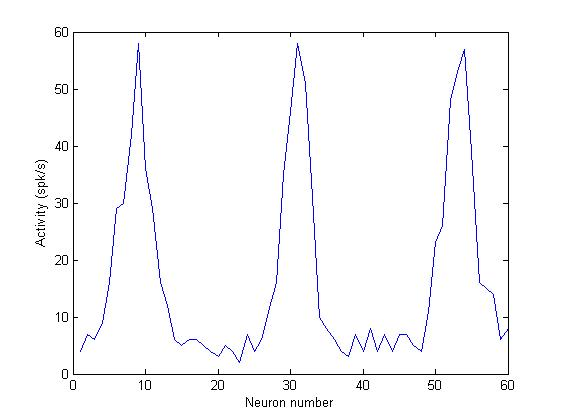
\includegraphics[width=90mm]{assignment1_images/31plot.jpg}
\caption{Plot of average firing rates for each neuron at the stimulus orientation}
\end{figure}

\begin{figure}[H]
\centering
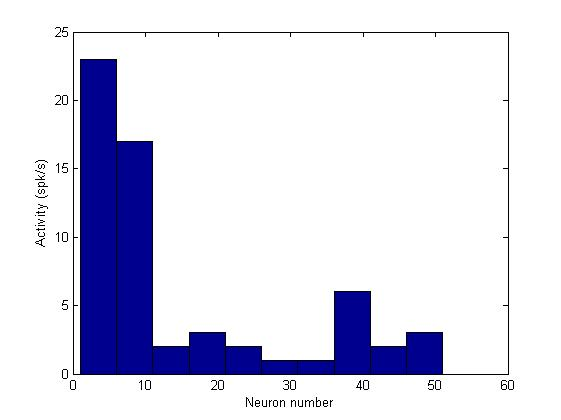
\includegraphics[width=90mm]{assignment1_images/31hist.jpg}
\caption{Histogram of the frequency of responses r}
\end{figure}

\section{Section 3.2}

\begin{figure}[H]
\centering
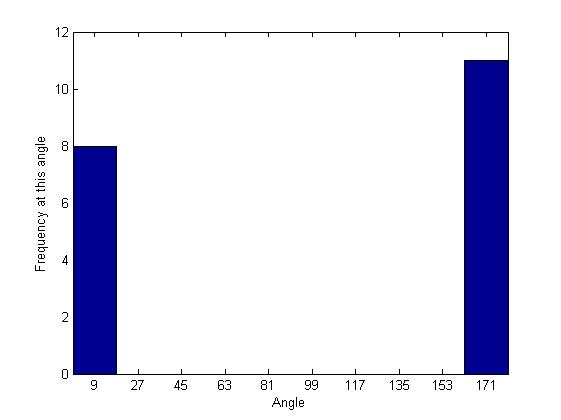
\includegraphics[width=90mm]{assignment1_images/32angles.jpg}
\caption{Results of varying stimulus}
\end{figure}

As we can see from the graph, there is a preference for neurons to converge to 180, showing a preference for horizontal stimulus. This result is independent on the the stimulus orientation. 


\end{document}